\section{Results and discussion}
\label{sec:results_discussion}
To study how the calculation of compressor map output uncertainty helps to determine the applicability of the map, the performance data of a $4.5 kW$ R22 reciprocating compressor listed in its manufacturer’s specification is used. The tabulated performance data shows the compressor power consumption at different evaporating and condensing temperature with a constant suction superheat 11 K within its operating range as shown in figure \ref{fig:oper_envelope}.

\begin{figure}[h]
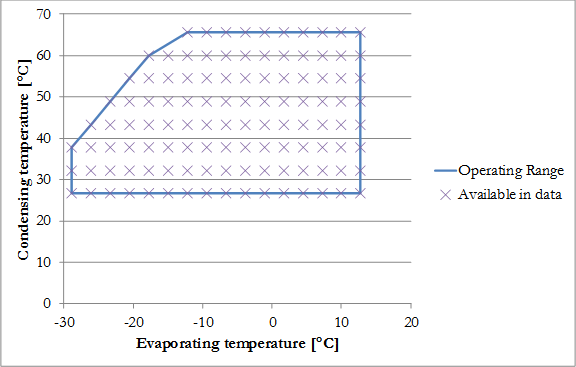
\includegraphics[width=0.7\linewidth]{./fig/operating_envelope.png}\hspace{0.05\linewidth}%
\begin{minipage}[b]{0.25\linewidth}\caption{\label{fig:oper_envelope}Operating envelope of compressor chosen for this study and available data points from manufacturer map.}
\end{minipage}
\end{figure}

Since the manufacturer data do not include experimental uncertainty, it is assumed that the data in the specification are the true values of the performance, and they are used to approximate the observations during steady state experiments with the assumptions in Table~\ref{tab:study_assumptions}.

\begin{table}[htbp]
  \centering
  \caption{Assumptions to approximate results in experiments of steady state compressor operation}
    \begin{tabular}{lcc}
    \toprule
    \textbf{Variable} & \textbf{Zero-order uncertainty} & \textbf{First-order uncertainty} \\
    \midrule
    Power consumption & 0.50\% & 3\% \\
    Evaporating pressure & 0.80\% & 0.9kPa \\
    Condensing pressure & 0.80\% & 0.4kPa \\
    \bottomrule
    \end{tabular}%
  \label{tab:study_assumptions}%
\end{table}%

The steady state experiment is assumed to have been conducted for 10 minutes with data acquired at 0.1Hz. The experimental observations at all data points in Figure~\ref{fig:oper_envelope} are generated by the method listed in section~\ref{sec:approx_uncertainty}.\\

\subsection{Study cases}
\label{sec:study_cases}

To examine if the applicability of compressor map changes with the conditions of the training data, various compressor maps trained from different ranges of data are compared. Six maps with different ranges of training data are designed for the study and the ranges of the training data in these maps are shown in Figure~\ref{fig:training_envelope}.


\begin{figure}[h]
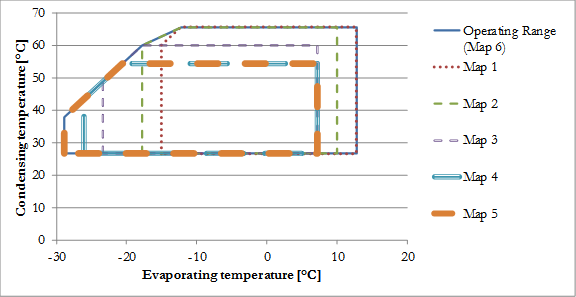
\includegraphics[width=0.7\linewidth]{./fig/training_data_sets.png}\hspace{0.05\linewidth}%
\begin{minipage}[b]{0.25\linewidth}\caption{\label{fig:training_envelope} Range of training data for different maps.}
\end{minipage}
\end{figure}

Figure~\ref{fig:training_envelope} shows that map 1 to 5 have their ranges of training data shifting from the top right-handed corner of the operating range of the compressor to its bottom left-handed corner, and map 6 covers the entire operating range. Since it is unfair to compare maps that are generated by different number of data points, the training data points in each map are arranged such that each map contains 70 data points.

\subsection{Comparison of maps}